\begin{frame}{Diapositiva con dos columnas}
    \begin{columns}
        \begin{column}{0.5\textwidth}
        \centering
        \textsc{Ecuación de Schrödinger en una columna}.
        \vspace{0.5cm}
        \begin{equation*}
            -\frac{\hbar^2}{2m}\nabla^2\psi + V\psi =  i\hbar\frac{\partial \psi}{\partial t}
        \end{equation*}
        \end{column}
        \vrule{}
        \begin{column}{0.5\textwidth}
            \centering
            \emph{\textrm{Imagen de un gato en la otra}}\\ [2ex]
            \centering
            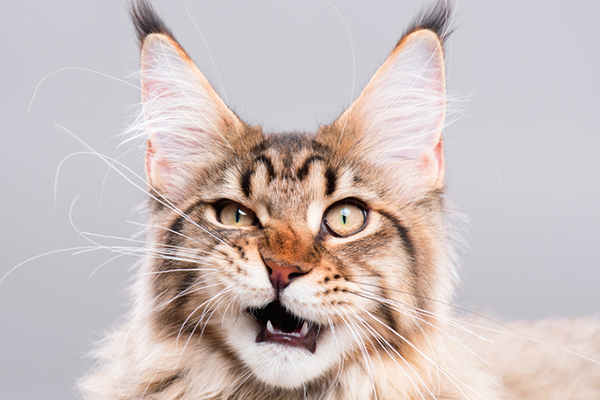
\includegraphics[width=0.8\linewidth]{gato.jpeg}
        \end{column}
    \end{columns}
\end{frame}